
%(BEGIN_QUESTION)
% Copyright 2007, Tony R. Kuphaldt, released under the Creative Commons Attribution License (v 1.0)
% This means you may do almost anything with this work of mine, so long as you give me proper credit

Two engineers propose different plans for adjustable ratio control in the following paint mixing system.  One of these schemes will work, but the other will prove to be unstable.  Which scheme is better, and why?

$$\includegraphics[width=15.5cm]{i01730x01.eps}$$

\vskip 10pt

$$\includegraphics[width=15.5cm]{i01730x02.eps}$$

Beware: this is a deep question!

\underbar{file i01730}
%(END_QUESTION)





%(BEGIN_ANSWER)

This is the more stable control system of the two:

$$\includegraphics[width=15.5cm]{i01730x02.eps}$$

The other control system was unstable because the gain of the flow control loop varied with the ``wild'' flow, as well as with the ratio setpoint.  If this is not immediately apparent (which it usually isn't to most), imagine a case where we were trying to maintain a 1:1 ratio with 50 GPM of pigment and 50 GPM of base, both flowmeters being ranged for 0-100 GPM.  A 1\% change in pigment flow would equate to a 2\% change in ratio (51 GPM base / 50 GPM pigment = 1.02 pigment:base ratio):

%(END_ANSWER)





%(BEGIN_NOTES)


%INDEX% Control, strategies: ratio
%INDEX% Process: paint mixing

%(END_NOTES)


